%% Manuscript draft -- target journal: Nuclear Instruments and Methods in
%% Physics Research A (Elsevier elsarticle class).
\documentclass[3p]{elsarticle}

\usepackage{amsmath,amssymb}
\usepackage{graphicx}
\usepackage{booktabs}
\usepackage{siunitx}
\usepackage{multirow}
\usepackage{xcolor}
\usepackage{subcaption}
\usepackage[hidelinks]{hyperref}

\graphicspath{{../report/figures/}}

\sisetup{detect-all}
\newcommand{\gfour}{Geant4}
\newcommand{\pe}{\ensuremath{N_{\mathrm{pe}}}}
\newcommand{\ngam}{\ensuremath{N_{\gamma}}}
\newcommand{\eps}{\ensuremath{\varepsilon}}
\newcommand{\sipm}{SiPM}

\journal{Nuclear Instruments and Methods in Physics Research A}

\begin{document}

\begin{frontmatter}

\title{A \gfour\ optical-photon simulation of light collection in a polished
plastic scintillator read out by side-coupled silicon photomultipliers for
muon trigger detectors}

\author[label1]{J. Turko\corref{cor1}}
\cortext[cor1]{Corresponding author}
\ead{}

\address[label1]{Institution, Address, City, Country}

\begin{abstract}
Plastic scintillator plates read out by silicon photomultipliers (\sipm{}s)
are candidates for large-area, low-cost muon trigger detectors in muon
tomography. We present a \gfour{} (v11.3.2) Monte Carlo model of a polished
polystyrene-based (polyvinyltoluene) scintillator plate of
\SI{250}{\milli\meter}$\times$\SI{250}{\milli\meter}$\times$\SI{10}{\milli\meter}
read out by \SI{4}{\milli\meter}$\times$\SI{4}{\milli\meter} side-coupled
\sipm{}s, reproducing the detector configurations and reflector treatments
reported by Rao \emph{et al.}\ [J.~Appl.\ Phys.\ \textbf{138}, 114504 (2025)].
The optical response is simulated with the \gfour{} unified surface model,
including scintillation and \v{C}erenkov generation, bulk absorption and
wavelength shifting. Photodetection is implemented through the wavelength-
dependent photon detection efficiency (PDE) of the \sipm{} photocathode, and
the bare plate is optically coupled to a black holder to represent frustrated
total internal reflection. A matrix of four \sipm{} layouts and four reflector
treatments is evaluated at three beam positions (48 runs, \num{48000} events),
together with a \num{25000}-event whole-plate scan. The simulation reproduces
the measured ordering of light collection,
$\text{bare} \ll \text{TiO}_2 < \text{Al} \approx \text{glossy}$, in every
layout, and predicts a position contrast below \SI{4}{\percent} for the
specular reflectors. The wavelength-shifting fibre configuration shifts the
mean detected wavelength from \SI{460}{\nano\meter} to \SI{485}{\nano\meter}.
The results quantify the role of the reflector in homogenising the response and
provide a validated optical model for the design of large-area trigger
detectors.
\end{abstract}

\begin{keyword}
Monte Carlo simulation \sep \gfour \sep plastic scintillator \sep
silicon photomultiplier \sep light collection \sep muon tomography
\end{keyword}

\end{frontmatter}

% =====================================================================
\section{Introduction}
\label{sec:intro}
% =====================================================================

Cosmic-ray muons are used to image large, dense objects in applications
ranging from volcano and pyramid surveys to the verification of spent nuclear
fuel in dry storage casks and to border security
\cite{Borozdin2003,Bonechi2020}. The mean muon energy at sea level is
approximately \SI{4}{\giga\electronvolt} and the flux is about
\SI{1}{cm^{-2}\,min^{-1}}, with a $\cos^2\theta$ zenith distribution; because
muons lose energy slowly, they traverse metre-scale shielding and their
scattering and absorption carry information about the material they cross
\cite{Rao2025}. Large-area plastic scintillator panels read out by
photomultipliers are the established technology for the trigger planes of such
systems. The transition from photomultiplier tubes (PMTs) to silicon
photomultipliers (\sipm{}s) is motivated by the low cost, low bias voltage,
compactness and mechanical robustness of \sipm{}s, which makes them attractive
for modular and mobile detectors \cite{Gundacker2020}. The principal
difficulty is the small active area of a \sipm{} compared with the area of the
scintillator plate and its dark count rate: the number of photoelectrons
produced by a muon must exceed the thermal noise baseline, which typically
requires a reflector treatment that retains and redirects scintillation light
towards the photosensors \cite{Rao2025}.

Rao \emph{et al.} \cite{Rao2025} have reported an experimental study of
\SI{250}{\milli\meter}$\times$\SI{250}{\milli\meter}$\times$\SI{10}{\milli\meter}
polished scintillator plates read out by side-coupled \sipm{}s, in four
configurations (eight, four and two \sipm{}s, and a single \sipm{} coupled to a
wavelength-shifting (WLS) fibre clamp) and with four surface treatments (bare,
white reflector paint, aluminium foil and high-gloss paper). They found that
reflective treatments raise the collected light yield by more than an order of
magnitude and that the high-gloss paper and aluminium foil perform best, and
they proposed the single-\sipm{} WLS-fibre configuration as a cost-effective
design for large-area detectors.

The present work develops an independent \gfour{} Monte Carlo model of the
same detector and uses it to reproduce the measured ordering of light
collection and to expose the photon-transport mechanisms behind it. Optical
photon tracking is difficult to model analytically because it is a many-bounce
random walk whose outcome depends on the surface finishes. We therefore
describe the geometry and optical parameters of every volume and surface, state
the physics processes used, and validate the model against the experimental
ordering. In addition to the three measurement positions of
Ref.~\cite{Rao2025}, a whole-plate scan is performed to quantify the spatial
uniformity of the response, which is a design-relevant quantity for a trigger
detector.

The article is organised as follows. Section~\ref{sec:methods} describes the
detector model, the optical parameters and the simulation campaign.
Section~\ref{sec:results} presents the collection efficiency, the photon
spectra and the spatial response. Section~\ref{sec:discussion} discusses the
physics interpretation and the limitations of the model, and
Section~\ref{sec:conclusions} concludes.

% =====================================================================
\section{Materials and methods}
\label{sec:methods}
% =====================================================================

\subsection{Detector model}
\label{sec:geometry}

The active volume is a polished polyvinyltoluene (PVT) scintillator plate of
\SI{250}{\milli\meter}$\times$\SI{250}{\milli\meter}$\times$\SI{10}{\milli\meter},
corresponding to the UPS-92S plate of Ref.~\cite{Rao2025} and representative of
the EJ-200 class \cite{EljenEJ200}. The plate is divided into a $100$-point
surface grid; its faces are either instrumented with \sipm{}s or covered by a
reflector. Each \sipm{} is modelled mechanically as a
\SI{4}{\milli\meter}$\times$\SI{4}{\milli\meter}$\times$\SI{0.6}{\milli\meter}
block of \sipm{} epoxy, coupled to the plate through a
\SI{0.1}{\milli\meter} layer of optical grease, so that the optical path is
plate\,$\rightarrow$\,grease\,$\rightarrow$\,\sipm{}. The sensors are placed as
siblings of the plate in the world volume and are clamped so that they do not
overhang the plate face.

Four layouts are studied, matching the four configurations of
Ref.~\cite{Rao2025} (Fig.~\ref{fig:layouts}):
\begin{description}
  \item[Config~1 (8 \sipm{}s):] two sensors on each of the four lateral faces,
    at $\pm 50\%$ of the half-length.
  \item[Config~2 (4 \sipm{}s):] one sensor on each face at the Config~1
    offsets.
  \item[Config~3 (2 \sipm{}s):] both sensors on the same face, at $\pm 50\%$,
    reproducing the T1/T2 arrangement of Ref.~\cite{Rao2025}.
  \item[Config~4 (1 \sipm{} + WLS fibre clamp):] a single sensor read out
    through four WLS fibres held in a machined clamp along one narrow face
    (Sec.~\ref{sec:wls}).
\end{description}

\begin{figure*}[t]
\centering
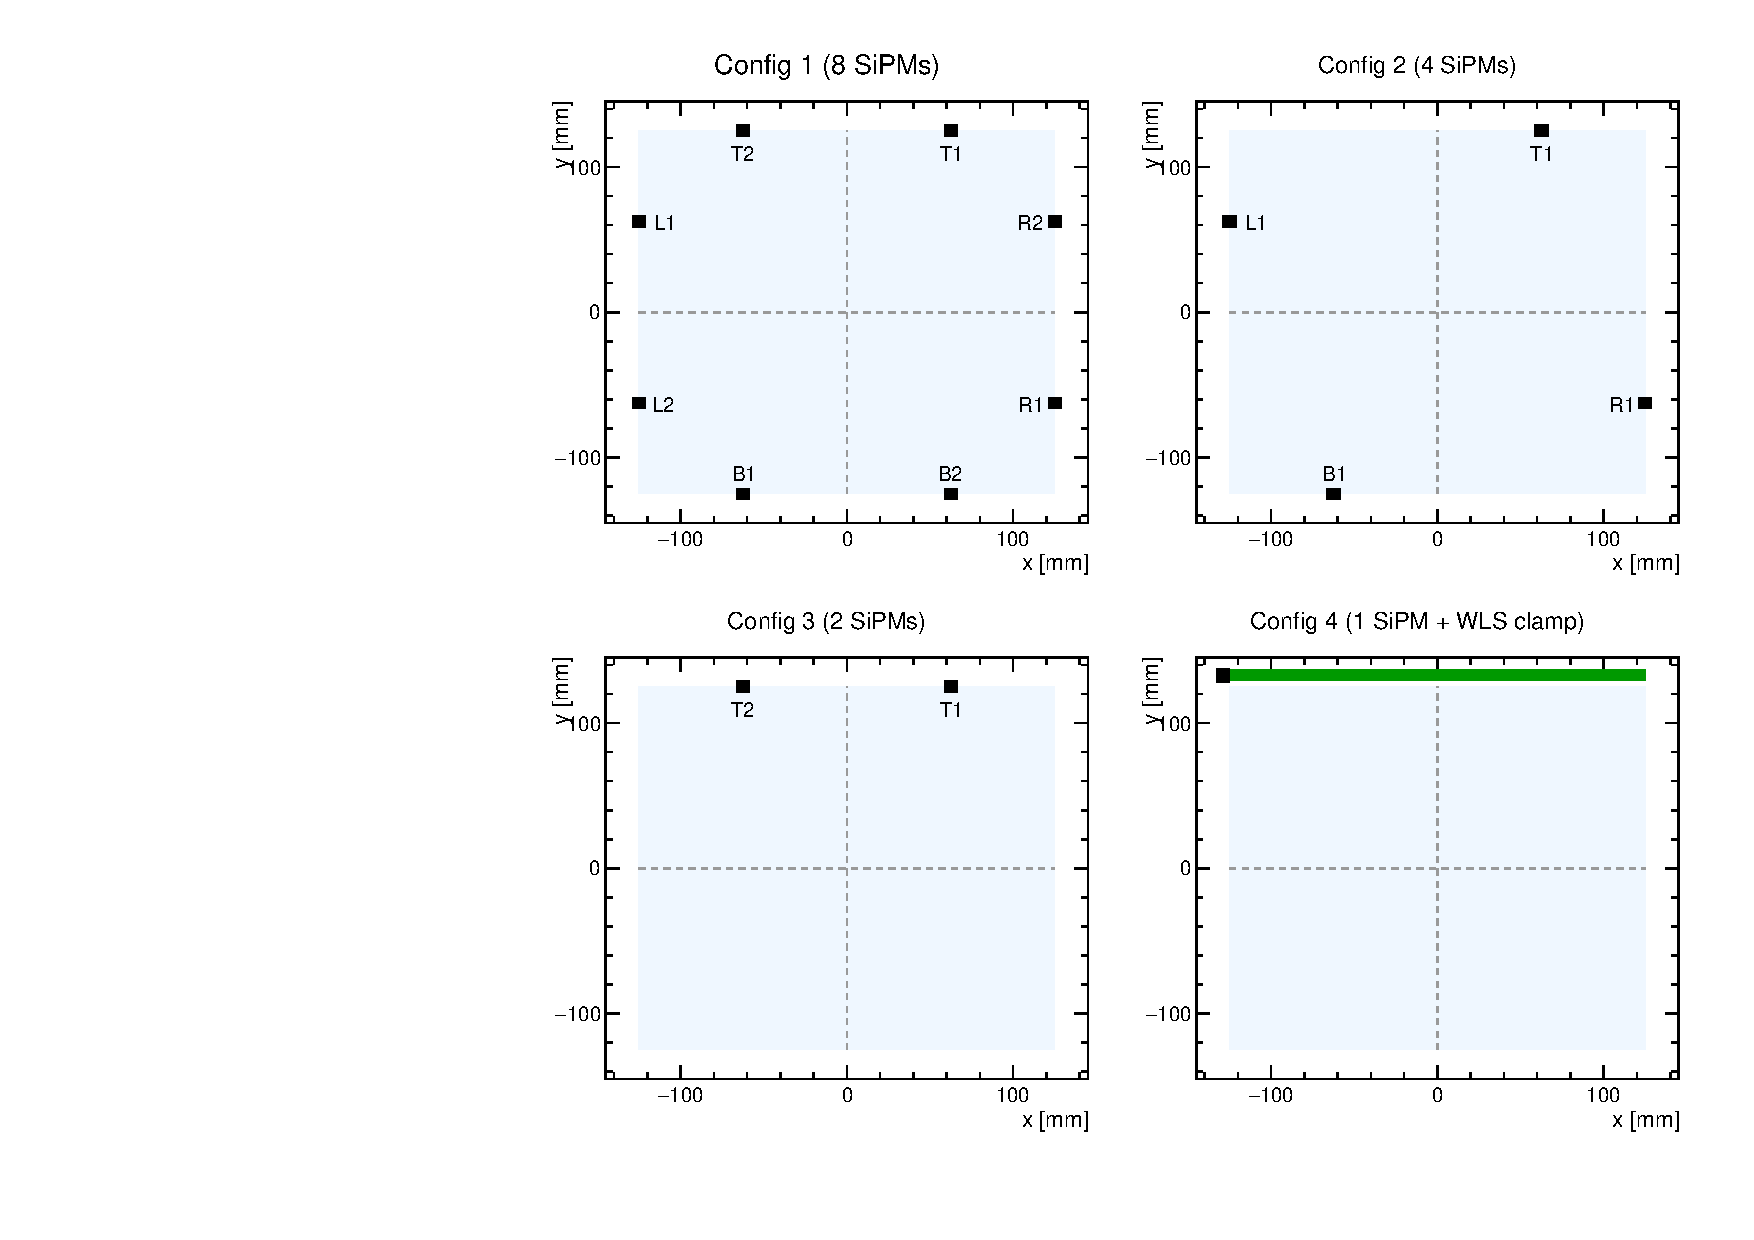
\includegraphics[width=0.6\textwidth]{sipm_layouts.pdf}
\caption{Schematic plan view of the four \sipm{} layouts on the
\SI{250}{\milli\meter}$\times$\SI{250}{\milli\meter} plate. Black squares mark
the side-mounted \sipm{}s (drawn oversized; the active area is
\SI{4}{\milli\meter}$\times$\SI{4}{\milli\meter}). Configs~1--3 use direct
coupling; Config~4 uses a single \sipm{} reading out a WLS fibre clamp along one
edge (green bar), with the read-out sensor at its end.}
\label{fig:layouts}
\end{figure*}

The non-instrumented faces receive one of four treatments: no reflector (the
plate is held in a black holder), white reflector paint, aluminium foil, or
high-gloss paper. The mapping from treatment to optical-surface parameters is
described in Sec.~\ref{sec:surfaces}.

\subsection{Optical parameters and surfaces}
\label{sec:surfaces}

Optical photons are transported with wavelength-dependent properties assigned
to every material and surface. The refractive index and bulk attenuation length
of the model materials are listed in Table~\ref{tab:materials}; the emission
spectrum is tabulated on the same grid. The scintillator emission peaks at
\SI{425}{\nano\meter}, and the bulk attenuation length has a maximum of
\SI{3.8}{\meter} that decreases steeply in the ultraviolet to represent
self-absorption. The \sipm{} photon detection efficiency is tabulated as a
function of wavelength, peaking at $0.43$ near \SI{425}{\nano\meter}, following
the ASD-NUV4S-P-40 device of Ref.~\cite{Rao2025}.

\begin{table}[t]
\centering
\caption{Refractive index $n$ and bulk attenuation length $L_{\mathrm{abs}}$
of the model materials. WLS = wavelength-shifting fibre.}
\label{tab:materials}
\small
\begin{tabular}{@{}llll@{}}
\toprule
Material & Role & $n$ & $L_{\mathrm{abs}}$ \\
\midrule
PVT scintillator        & active volume          & 1.58 & \SI{3.8}{\meter} (peak) \\
Optical grease          & plate--\sipm{} coupling & 1.46 & --- \\
\sipm{} epoxy            & photosensor body      & 1.55 & --- \\
Black holder            & light-tight enclosure  & 1.55 & \SI{1}{\micro\meter} \\
WLS fibre core          & Y-11(200) core         & 1.59 & \SI{5}{\meter} \\
WLS fibre cladding      & fibre cladding         & 1.49 & \SI{20}{\meter} \\
Fibre-clamp body        & black clamp            & 1.55 & \SI{1}{\micro\meter} \\
\bottomrule
\end{tabular}
\end{table}

The reflector treatments are implemented as logical surface skins applied to
the plate faces, using the \gfour{} unified surface model
\cite{Levin1996,Nilsson2015}. The parameters are summarised in
Table~\ref{tab:surfaces}. The white paint is modelled as a front-painted
Lambertian surface with reflectivity between $0.955$ and $0.983$; aluminium
foil and glossy paper are modelled as back-painted surfaces with a specular
spike, i.e.\ as mirrors, with reflectivities of $0.84$--$0.91$ and
$0.90$--$0.955$, respectively. This choice reflects the experimental result
that aluminium and glossy paper are the brightest treatments: a purely diffuse
model of glossy paper does not reproduce the observation, whereas a slightly
lossy mirror does.

\begin{table}[t]
\centering
\caption{Optical-surface model for the four reflector treatments. $R$ is the
tabulated reflectivity over \SIrange{360}{650}{\nano\meter}. All surfaces use
the unified model.}
\label{tab:surfaces}
\small
\begin{tabular}{@{}llll@{}}
\toprule
Treatment & \gfour{} type & \gfour{} finish & Reflectivity $R$ \\
\midrule
Bare / black holder & \texttt{dielectric\_dielectric} & \texttt{polished} (absorber) & $T=R=0$ \\
White paint (TiO$_2$)& \texttt{dielectric\_dielectric} & \texttt{groundfrontpainted} & $0.955$--$0.983$, Lambertian \\
Aluminium foil       & \texttt{dielectric\_dielectric} & \texttt{polishedbackpainted} & $0.84$--$0.91$, specular \\
Glossy paper         & \texttt{dielectric\_dielectric} & \texttt{polishedbackpainted} & $0.90$--$0.955$, specular \\
\bottomrule
\end{tabular}
\end{table}

The bare configuration requires particular care. A polished plate surrounded by
air traps light by total internal reflection (TIR) and would therefore be the
most efficient light guide, which contradicts the measurement in which the bare
plate gives the weakest signal. In the experiment the plate is mounted in a
black 3D-printed holder whose refractive index is close to that of the
scintillator; the faces are then in effective optical contact and TIR is
frustrated, so that trapped light leaks into the absorbing walls. This is
represented in the model by an absorber skin with $R=T=0$ on the plate faces
and a matching skin on the black holder. The same absorber skin is retained on
the five non-instrumented faces of Config~4.

Photodetection is delegated to the boundary process rather than drawn in the
sensitive detector. The grease--\sipm{} boundary is modelled as a
\texttt{dielectric\_metal} surface whose efficiency equals the \sipm{} PDE and
whose reflectivity is zero. When a photon reaches this boundary, the boundary
process performs the absorption draw, assigns the status \texttt{Detection} and
invokes the sensitive detector; the sensitive detector records one
photoelectron and terminates the photon. The \gfour{} option
\texttt{SetBoundaryInvokeSD(true)} is enabled for this purpose. The
plate--grease boundaries are transparent Fresnel surfaces, so that the coupling
chain is governed by the refractive-index mismatch alone.

\subsection{Config~4: WLS fibre clamp}
\label{sec:wls}

Config~4 follows the single-\sipm{}, WLS-fibre read-out of
Ref.~\cite{Rao2025}. Four Y-11(200) fibres of \SI{1.0}{\milli\meter} diameter
run along one narrow face over its full \SI{250}{\milli\meter} length at a
\SI{1.5}{\milli\meter} pitch and converge, over the last
\SI{15}{\milli\meter}, to a touching \SI{1.0}{\milli\meter} bundle that
presents all four ends to a single \sipm{}. The far ends are closed by
aluminium mirror caps. The fibres are held in a black clamp with a
\SI{1.1}{\milli\meter} channel per fibre, separated from the plate by a
\SI{0.10}{\milli\meter} grease film; each fibre protrudes
\SI{0.05}{\milli\meter} into the film so that the grease remains continuous
against the scintillator. The \SI{0.05}{\milli\meter} air annulus between the
\SI{1.0}{\milli\meter} fibre and its channel is retained because the modelled
cladding index ($n=1.49$) exceeds the grease index ($n=1.46$) only slightly; a
snug fit against the clamp would frustrate core--cladding TIR. The fibres are
built as tessellated swept cylinders and placed as world siblings of the plate.
The \gfour{} WLS process is enabled automatically for this geometry.

\subsection{Physics processes and Monte Carlo implementation}
\label{sec:physics}

The simulation uses \gfour{} v11.3.2 \cite{Agostinelli2003,Allison2016} with a
modular physics list built from the standard electromagnetic, hadronic elastic
and inelastic, thermal-neutron, ion and radioactive-decay constructors. Optical
photons are produced by the scintillation and \v{C}erenkov processes and
transported with bulk absorption, Rayleigh scattering and boundary processes
enabled; Mie scattering is disabled. Scintillation is described by a single
fast component with a decay time of \SI{2.1}{\nano\second} and a light yield of
\num{1.0e4} photons per \si{\mega\electronvolt}; the energy dependence of the
light yield is modelled with Birks' law with a constant of
\SI{0.126}{\milli\meter\per\mega\electronvolt}
\cite{Birks1951,Craun1970}. The boundary process requires a refractive index on
both sides of an interface; every material in the model therefore carries an
explicit refractive-index table, and a missing index would silently terminate
the photon. The wavelength-shifting process is enabled only for the Config~4
geometry and is inactive for all other layouts.

The implementation of the optical surfaces was verified against the \gfour{}
source. Reading the boundary process, a logical border surface between two
volumes takes precedence over a logical skin surface at the same boundary, and
a boundary with no surface object falls back to lossless TIR. These two
properties are used deliberately: the grease and \sipm{} patches punch holes in
the reflector skin, and the bare plate is given an absorber skin rather than a
reflective one.

\subsection{Simulation campaign and efficiency definition}
\label{sec:campaign}

The primary source is a vertical \SI{4}{\giga\electronvolt} $\mu^-$ pencil
beam, generated with the \gfour{} General Particle Source (GPS), with a square
cross-section of \SI{50}{\milli\meter}$\times$\SI{50}{\milli\meter} matching
the active area of the muon coincidence detector (MCD) of
Ref.~\cite{Rao2025}. Three irradiation positions are used, each illuminating a
\SI{50}{\milli\meter}$\times$\SI{50}{\milli\meter} patch lying entirely on the
plate: the centre, an edge mid-point, and a corner. The
edge and corner patches lie on the face opposite the instrumented face of the
single-sided layouts. The full matrix comprises four layouts, four reflector
treatments and three positions, i.e.\ $48$ runs of \num{1000} events each. A
second, whole-plate campaign replaces the pencil beam with a
\SI{250}{\milli\meter}$\times$\SI{250}{\milli\meter} beam so that the muon
entry point is sampled uniformly over the plate; \num{25000} events are
generated for each (layout, reflector) pair. All runs are executed with eight
threads and without biasing.

For a set of \sipm{}s $\mathcal{S}$ the collection efficiency is defined as
\begin{equation}
  \eps = \frac{\displaystyle\sum_{e}\sum_{s\in\mathcal{S}} \pe^{(e,s)}}
             {\displaystyle\sum_{e}\ngam^{(e)}},
  \label{eq:eff}
\end{equation}
where $\pe^{(e,s)}$ is the number of photoelectrons detected in sensor $s$ in
event $e$ and $\ngam^{(e)}$ is the total number of optical photons generated in
the plate during that event (scintillation and \v{C}erenkov). The numerator and
denominator are accumulated per event, so that the efficiency is a ratio of
sums and is independent of the number of sensors.

A dedicated diagnostic record accumulates, per event, the number of generated,
detected, escaped and terminated optical photons, the per-event produced-photon
count and the primary muon's first entry position in the plate. At the end of
each event the sensitive detector writes one row per (event, sensor), including
sensors with zero detections; the sample is therefore unbiased in the muon
interaction position. Each row carries the entry position, the produced-photon
count, the detected count, the first arrival time and the mean detected
wavelength. Position-resolved efficiencies are reconstructed offline from this
record in \SI{5}{\milli\meter} (matrix) or \SI{10}{\milli\meter} (whole plate)
cells.

% =====================================================================
\section{Results}
\label{sec:results}
% =====================================================================

\subsection{Collection efficiency}
\label{sec:eff}

Figure~\ref{fig:effbars} shows the simulated collection efficiency,
Eq.~\eqref{eq:eff}, summed over all \sipm{}s and over the three irradiation
positions, for every (layout, reflector) pair; the values are listed in
Table~\ref{tab:eff}. In every layout the ordering is
\begin{equation}
  \text{bare} \ll \text{TiO}_2 < \text{Al} \approx \text{glossy},
  \label{eq:ordering}
\end{equation}
which reproduces the experimental result of Ref.~\cite{Rao2025}. The bare plate
is suppressed by two orders of magnitude or more relative to the reflective
treatments, as expected for a surface whose faces are in effective optical
contact with an absorber. Aluminium and glossy paper are the most efficient
treatments and are indistinguishable within the statistical precision of the
sample. The efficiency increases with the number of sensors: Config~1 (eight
\sipm{}s) is the most efficient, followed by Config~2 (four) and Config~3
(two). The single-\sipm{} WLS-fibre layout (Config~4) collects the least light,
since only the fraction of photons that reach the fibre face is converted and
guided to the sensor.

\begin{figure*}[t]
\centering
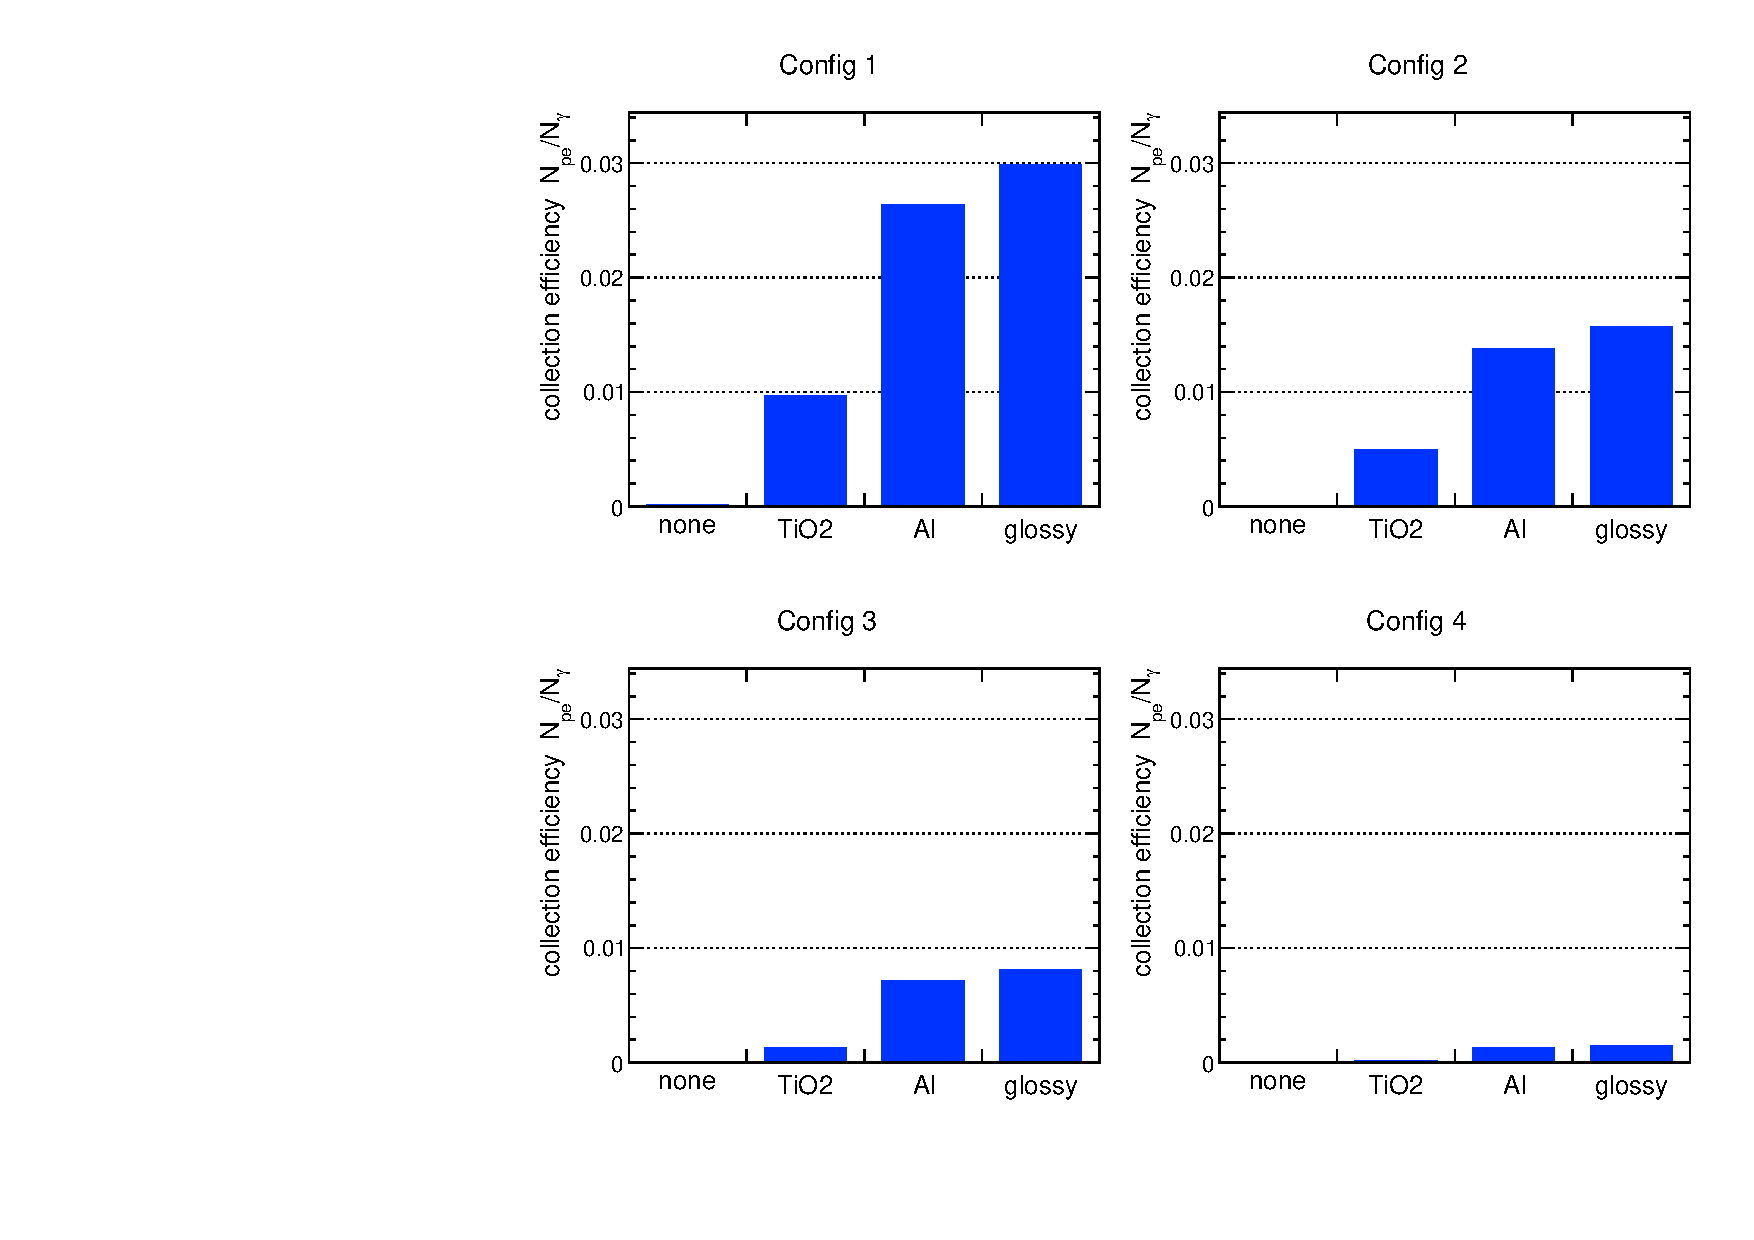
\includegraphics[width=0.7\textwidth]{fig_eff_bars.pdf}
\caption{Simulated collection efficiency, Eq.~\eqref{eq:eff}, for the four
reflector treatments and four \sipm{} layouts. The ordering
$\text{bare} \ll \text{TiO}_2 < \text{Al} \approx \text{glossy}$ is reproduced in
every layout.}
\label{fig:effbars}
\end{figure*}

\begin{table}[t]
\centering
\caption{Simulated collection efficiency (all \sipm{}s and all irradiation
positions combined).}
\label{tab:eff}
\small
\begin{tabular}{@{}lcccc@{}}
\toprule
Layout & Bare & TiO$_2$ & Al & Glossy \\
\midrule
Config~1 (8 \sipm{}s)      & $1.9\times10^{-4}$ & $9.7\times10^{-3}$ & $2.64\times10^{-2}$ & $2.99\times10^{-2}$ \\
Config~2 (4 \sipm{}s)      & $9.6\times10^{-5}$ & $4.9\times10^{-3}$ & $1.38\times10^{-2}$ & $1.58\times10^{-2}$ \\
Config~3 (2 \sipm{}s)      & $2.4\times10^{-5}$ & $1.30\times10^{-3}$ & $7.20\times10^{-3}$ & $8.18\times10^{-3}$ \\
Config~4 (1 \sipm{}, WLS)  & $6.9\times10^{-6}$ & $2.2\times10^{-4}$ & $1.35\times10^{-3}$ & $1.47\times10^{-3}$ \\
\bottomrule
\end{tabular}
\end{table}

\subsection{Photon yield and photoelectron spectra}
\label{sec:spectra}

Figure~\ref{fig:spectra}(a) shows the per-event optical-photon yield (the
denominator of Eq.~\eqref{eq:eff}) for the four treatments. The mean yield is
essentially independent of the reflector, at approximately \num{19000} photons
per event, as required: the reflector changes the transport of photons, not
their production. The residual spread reflects the event-to-event variation of
the muon path length for a vertical beam of fixed cross-section.
Figure~\ref{fig:spectra}(b) shows the corresponding photoelectron spectra, in
which the reflector has a decisive effect. The bare configuration peaks near
zero, with a mean of \num{3.7} photoelectrons per event for Config~1, whereas
glossy paper gives a mean of \num{586} photoelectrons per event. The transition
from a near-zero-peaked to a broad distribution is the direct signature of
efficient light collection. With approximately \num{19000} photons produced and
$\approx 586$ photoelectrons detected, the collection efficiency is
$\approx \SI{3}{\percent}$, consistent with the \sipm{} PDE of
$\approx 0.43$ and the geometric acceptance of a side-coupled sensor.

\begin{figure*}[t]
\centering
\begin{subfigure}{0.49\textwidth}
  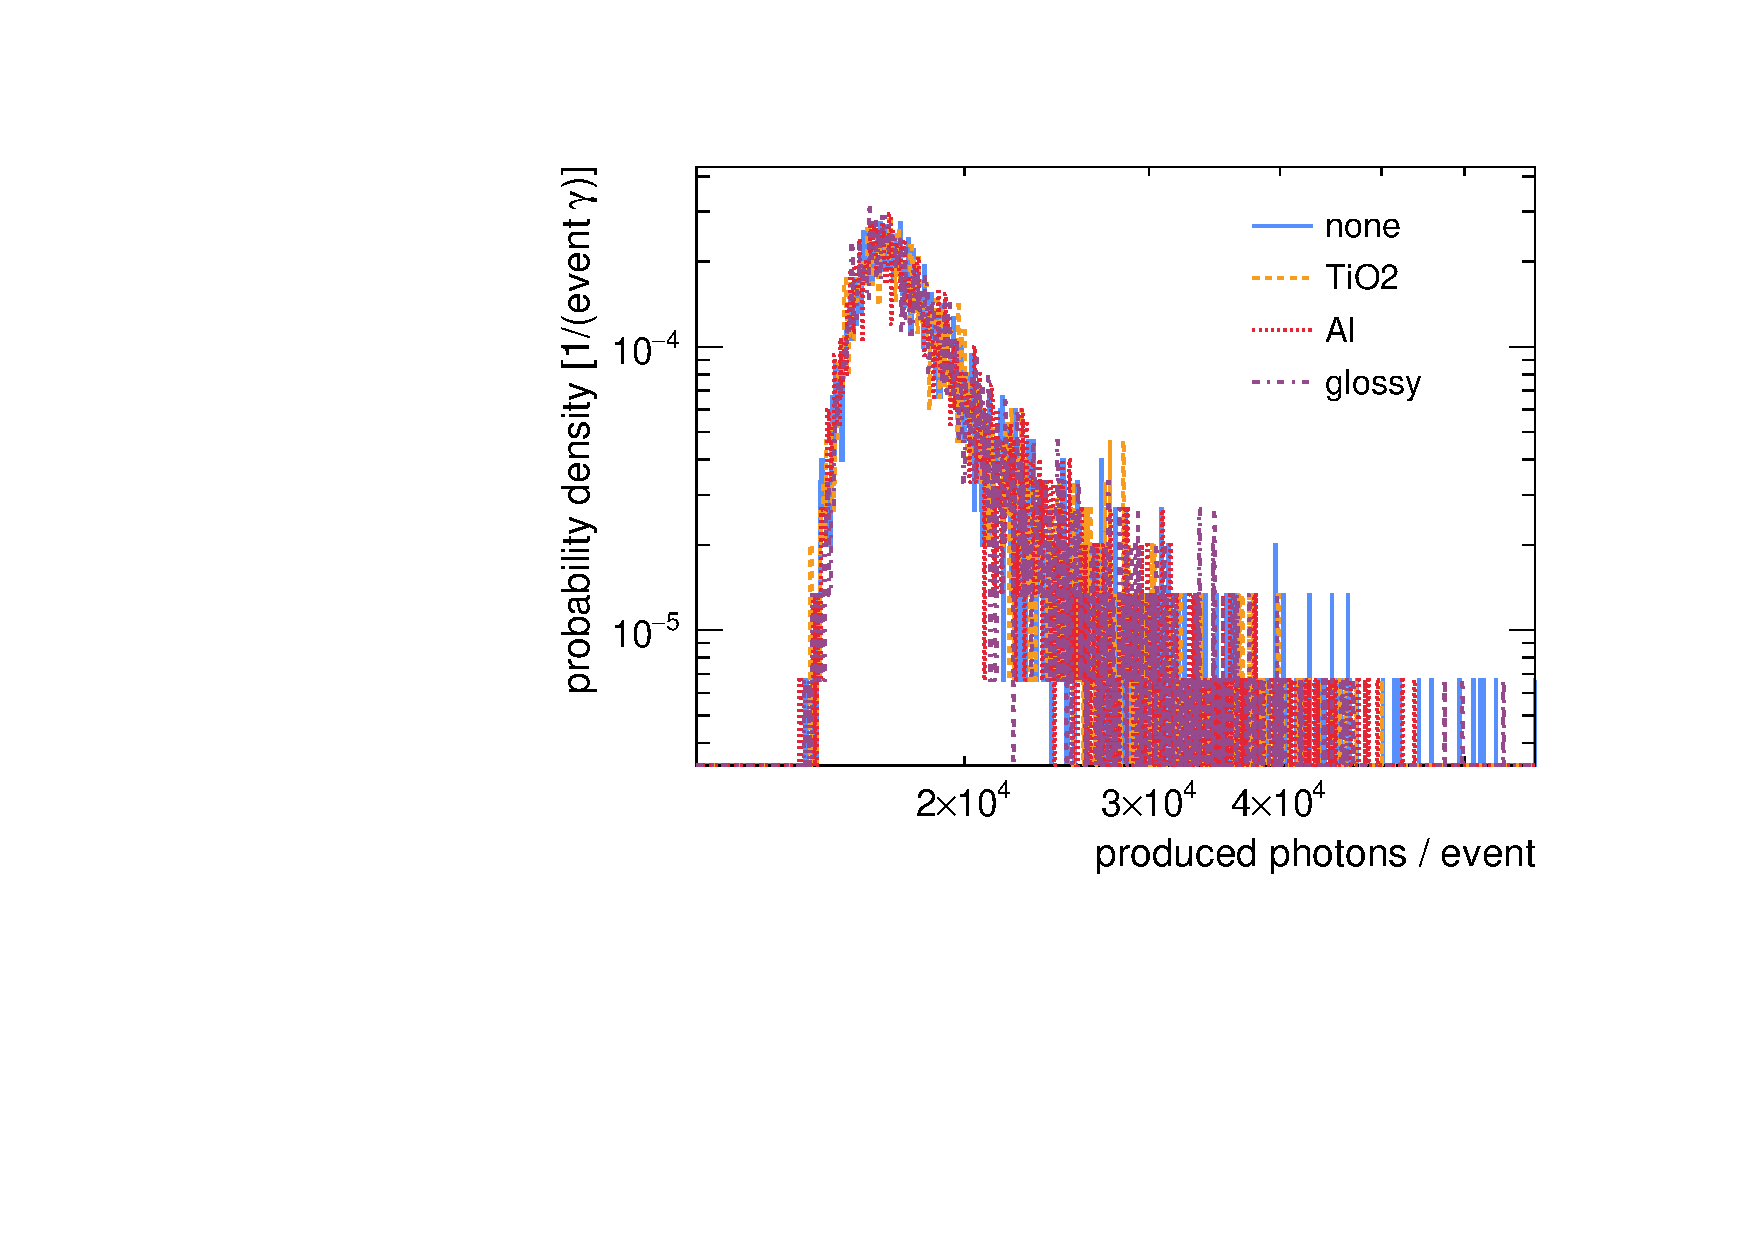
\includegraphics[width=\linewidth]{fig_yield.pdf}
  \caption{Produced optical photons per event.}
\end{subfigure}\hfill
\begin{subfigure}{0.49\textwidth}
  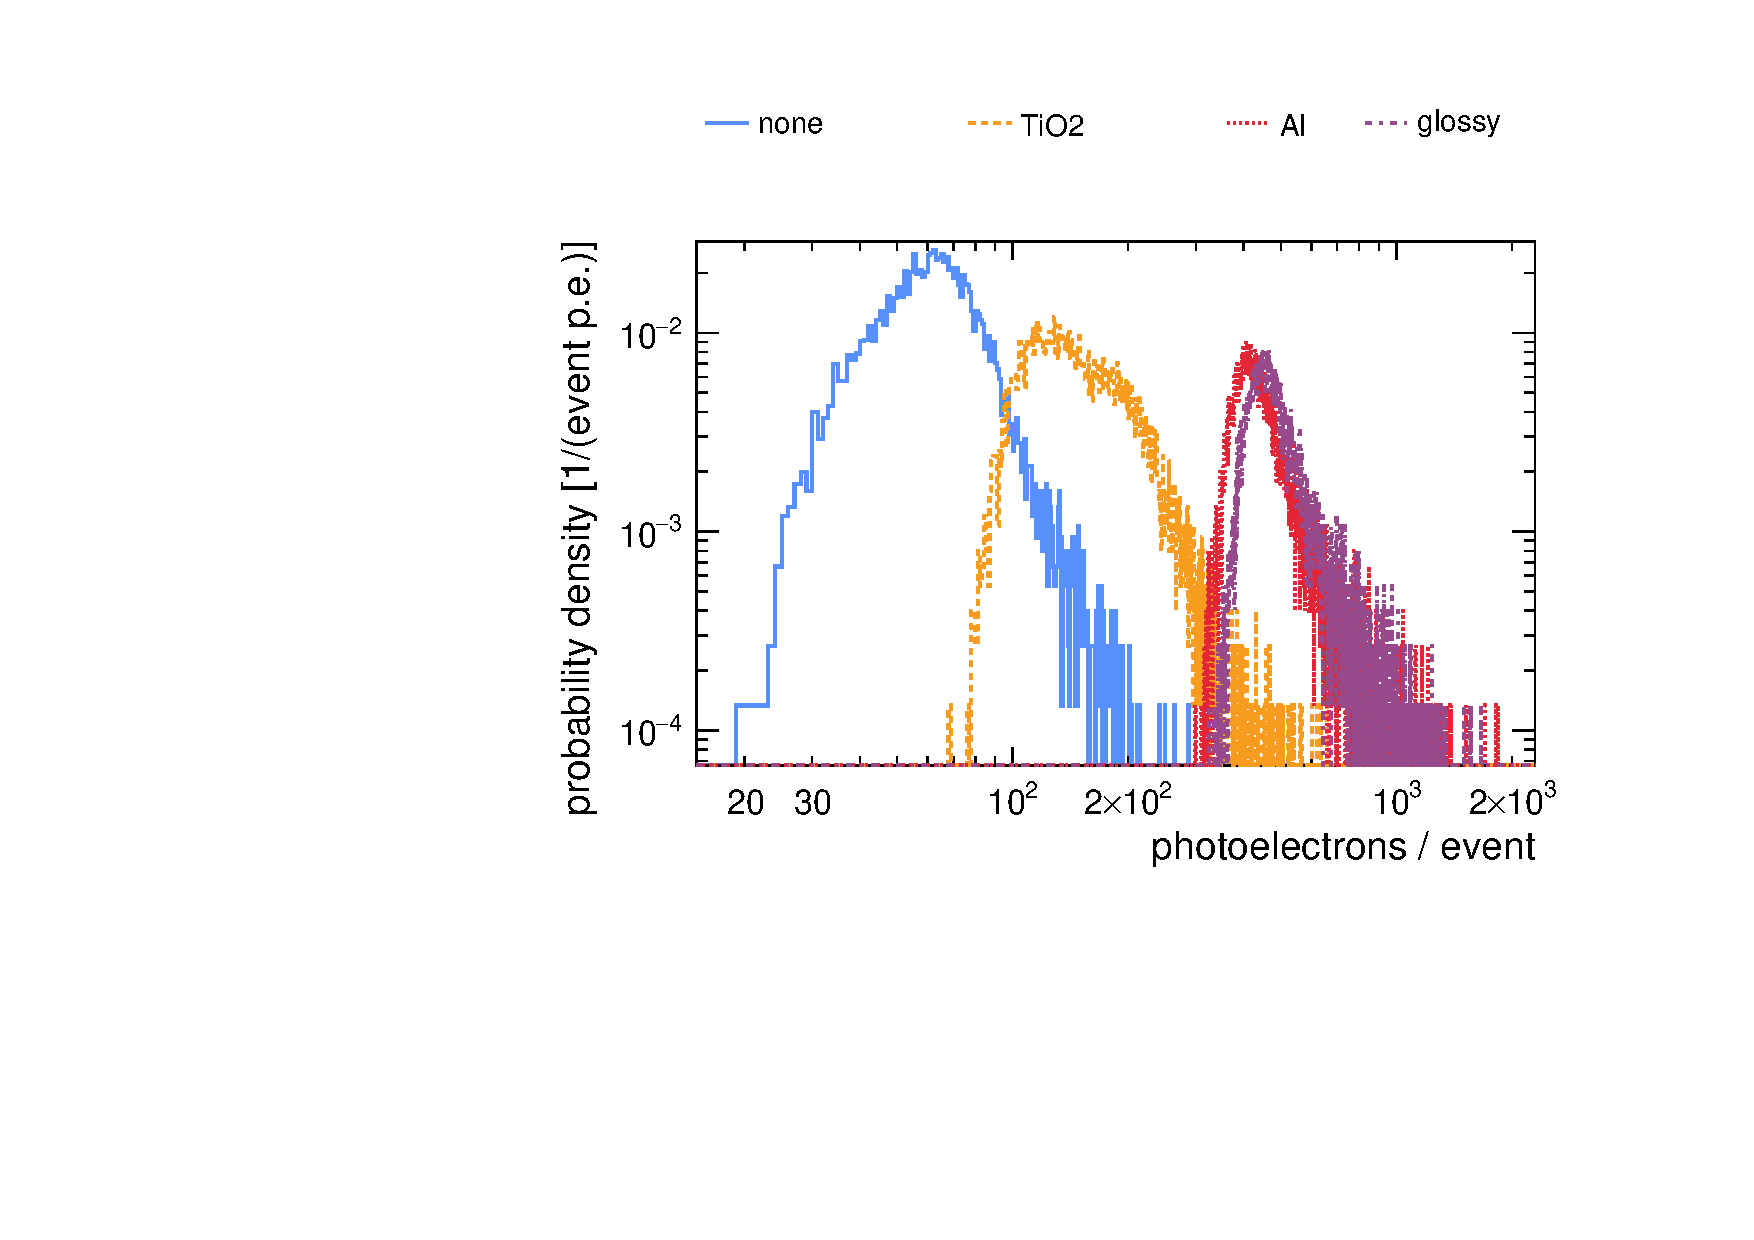
\includegraphics[width=\linewidth]{fig_detected.pdf}
  \caption{Detected photoelectrons per event.}
\end{subfigure}
\caption{Per-event distributions for Config~1 (unit-area probability density;
logarithmic axes): (a) the production yield is reflector-independent, while
(b) the detected photoelectron count depends strongly on the reflector.}
\label{fig:spectra}
\end{figure*}

\subsection{Detected wavelength}
\label{sec:wavelength}

Figure~\ref{fig:wavelength} shows the wavelength distribution of the detected
photoelectrons for each treatment and layout. Configs~1--3, which couple the
\sipm{}s directly to the plate, detect the same blue scintillation spectrum;
the mean wavelength varies only from \SI{459.8}{\nano\meter} (glossy, Config~1)
to \SI{460.1}{\nano\meter} (Config~3). The spectrum is red-shifted with respect
to the \SI{425}{\nano\meter} emission peak because the short-wavelength part of
the emission overlaps the absorption band and is attenuated over the
multi-bounce path. Config~4 is qualitatively different: the WLS fibres absorb
the blue light and re-emit it at their own emission band, shifting the mean
detected wavelength to \SI{485.2}{\nano\meter} (glossy), a shift of
approximately \SI{25}{\nano\meter}. The same shift appears for every treatment,
confirming that it originates in the fibre wavelength shifter rather than in the
reflector.

\begin{figure*}[t]
\centering
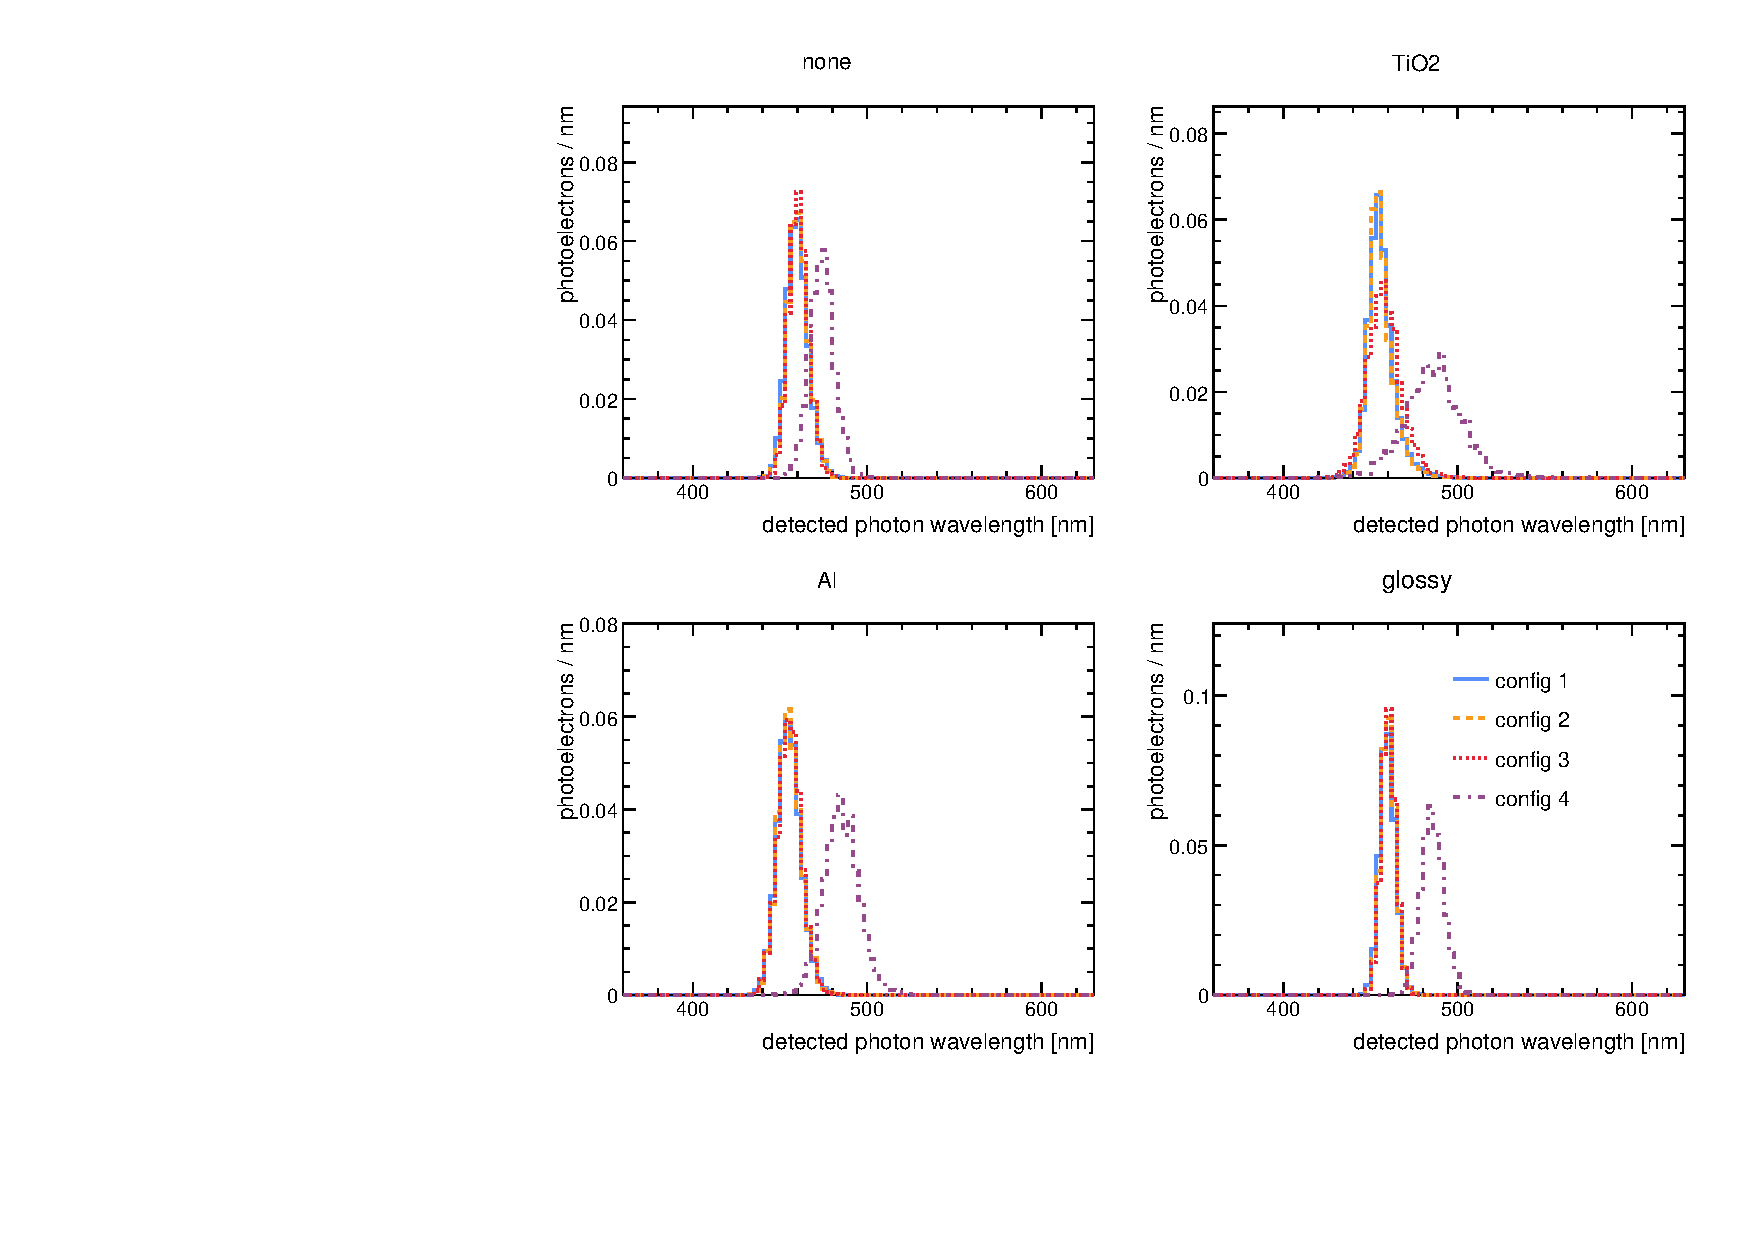
\includegraphics[width=0.65\textwidth]{fig_wavelength_cfg.pdf}
\caption{Detected-photon wavelength distribution, weighted by photoelectron
count, for each reflector (panel) and each layout (curves). Configs~1--3 follow
the blue scintillation spectrum near \SI{460}{\nano\meter}, whereas the
WLS-fibre read-out of Config~4 is shifted to approximately
\SI{485}{\nano\meter}.}
\label{fig:wavelength}
\end{figure*}

\subsection{Position dependence and light sharing}
\label{sec:position}

The three irradiation patches have equal area and lie entirely on the plate, so
their produced-photon denominators are equal and their efficiencies are
directly comparable. Figure~\ref{fig:pos} presents the efficiency at the
centre, edge and corner for each layout. The reflective treatments homogenise
the response: for aluminium and glossy paper the efficiency varies by less than
\SI{4}{\percent} across the three patches in every layout. The diffuse
TiO$_2$ paint is less uniform, and the bare plate shows the strongest position
dependence. This behaviour is quantified by the position contrast
\begin{equation}
  \kappa = \frac{\eps_{\max}}{\eps_{\min}},
  \label{eq:contrast}
\end{equation}
the ratio of the largest to the smallest patch-averaged efficiency, listed in
Table~\ref{tab:contrast}. The mirror-like treatments hold $\kappa \le 1.03$,
whereas $\kappa$ reaches $1.7$--$2.1$ for TiO$_2$ and up to $3.7$ for the bare
plate. The result is that a closed reflective cavity retains little memory of
the muon entry point after a few bounces; the sensor coverage, rather than the
irradiation position, then sets the collection efficiency.

\begin{figure*}[t]
\centering
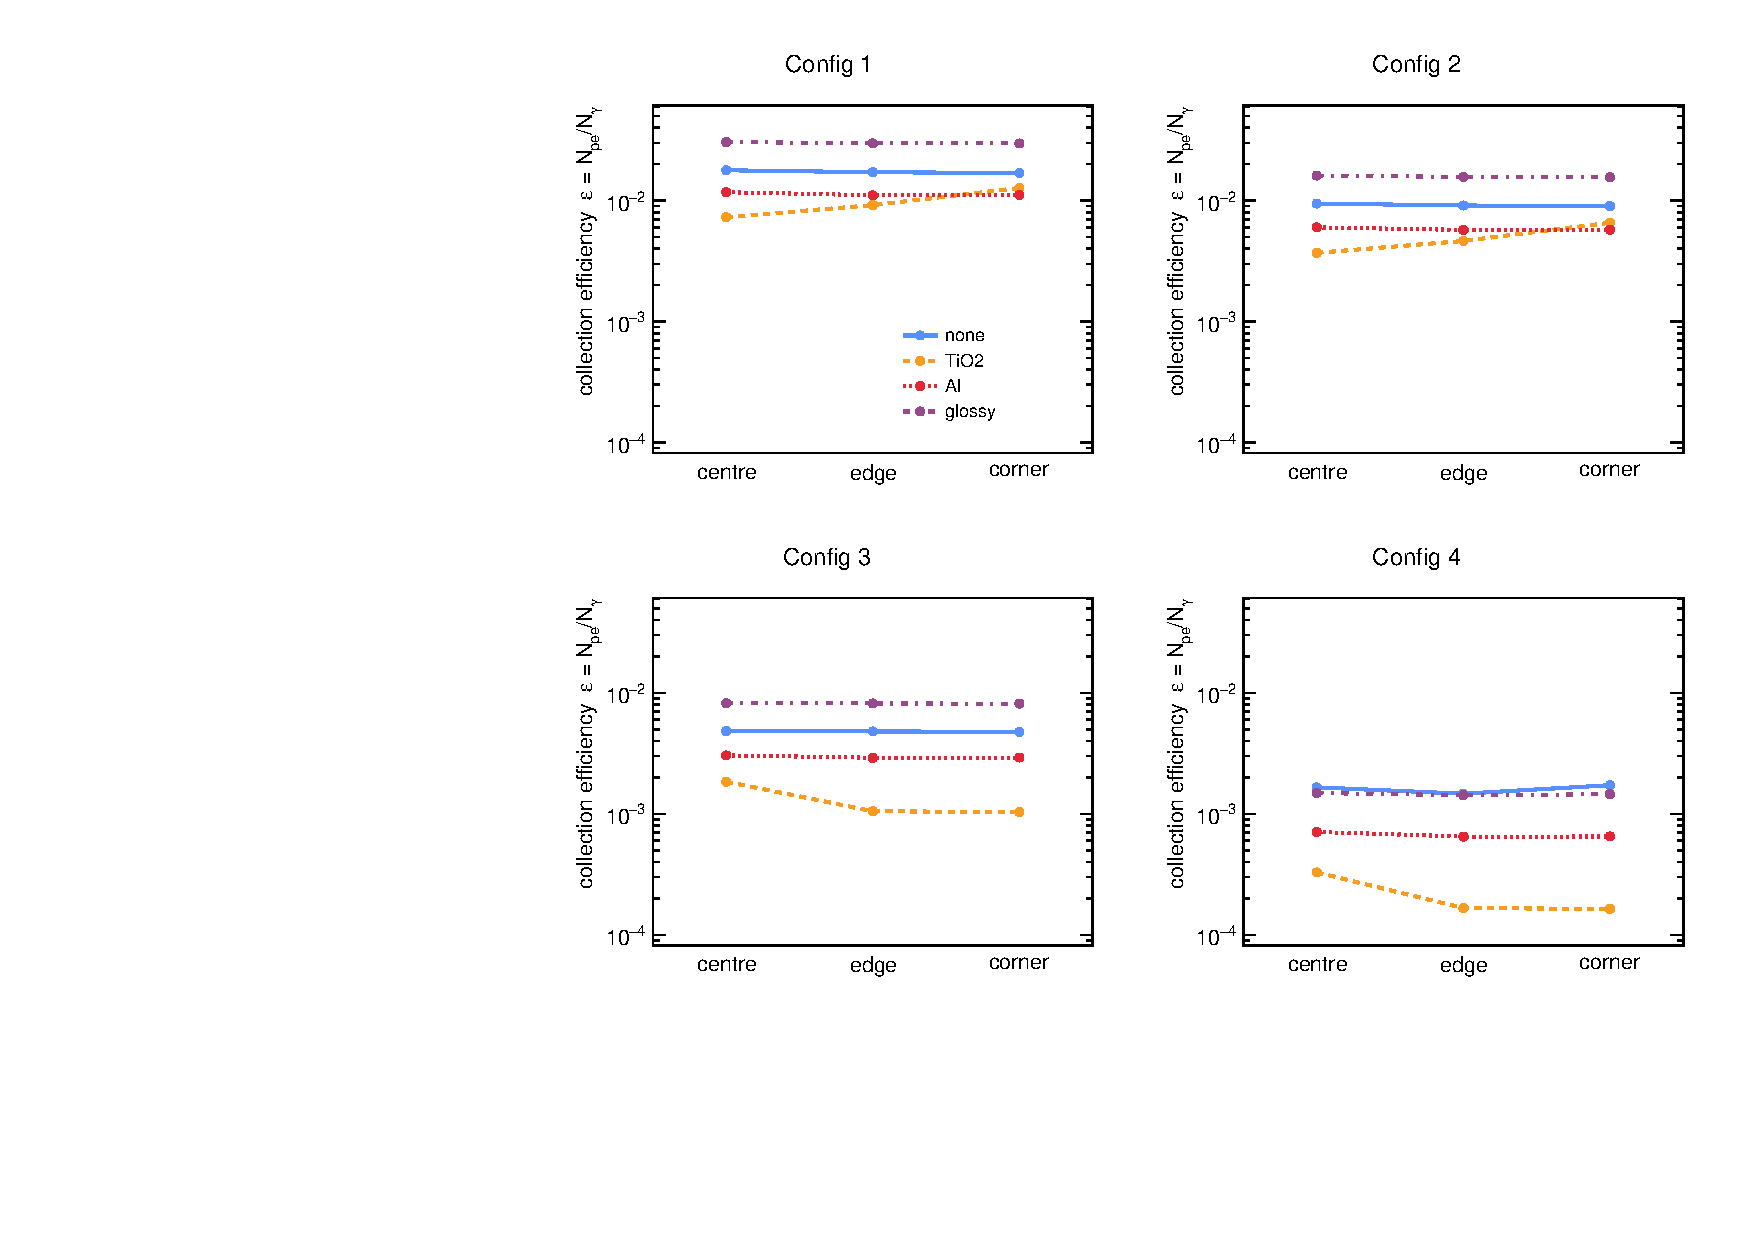
\includegraphics[width=0.7\textwidth]{fig_pos_layouts.pdf}
\caption{Collection efficiency at the centre, edge and corner patches, one
panel per layout, for the four treatments (logarithmic axis). The reflective
treatments are nearly flat across the three patches, whereas the bare plate is
both the weakest and the most position-dependent.}
\label{fig:pos}
\end{figure*}

\begin{table}[t]
\centering
\caption{Position contrast $\kappa=\eps_{\max}/\eps_{\min}$
(Eq.~\eqref{eq:contrast}) across the three irradiation patches.}
\label{tab:contrast}
\small
\begin{tabular}{@{}lcccc@{}}
\toprule
Treatment & Config~1 & Config~2 & Config~3 & Config~4 \\
\midrule
Bare    & 2.22 & 1.98 & 3.33 & 3.73 \\
TiO$_2$ & 1.74 & 1.72 & 1.81 & 2.09 \\
Al      & 1.03 & 1.03 & 1.01 & 1.03 \\
Glossy  & 1.03 & 1.03 & 1.00 & 1.03 \\
\bottomrule
\end{tabular}
\end{table}

Figure~\ref{fig:sharing} resolves the directional response for Config~1 by
showing the share of the collected light detected by each of the eight sensors.
For the bare plate at the corner patch, the two sensors nearest the beam
collect \SI{91}{\percent} of all photoelectrons, approximately $3.6$ times the
uniform share each, while two of the remaining sensors record nothing. A
reflective treatment removes this structure: for glossy paper the same two
sensors reach only about $1.1$ times the uniform share. The total efficiency is
nearly the same for all three patches, so the cavity keeps the amount of
collected light constant while redistributing it among the sensors.

\begin{figure*}[t]
\centering
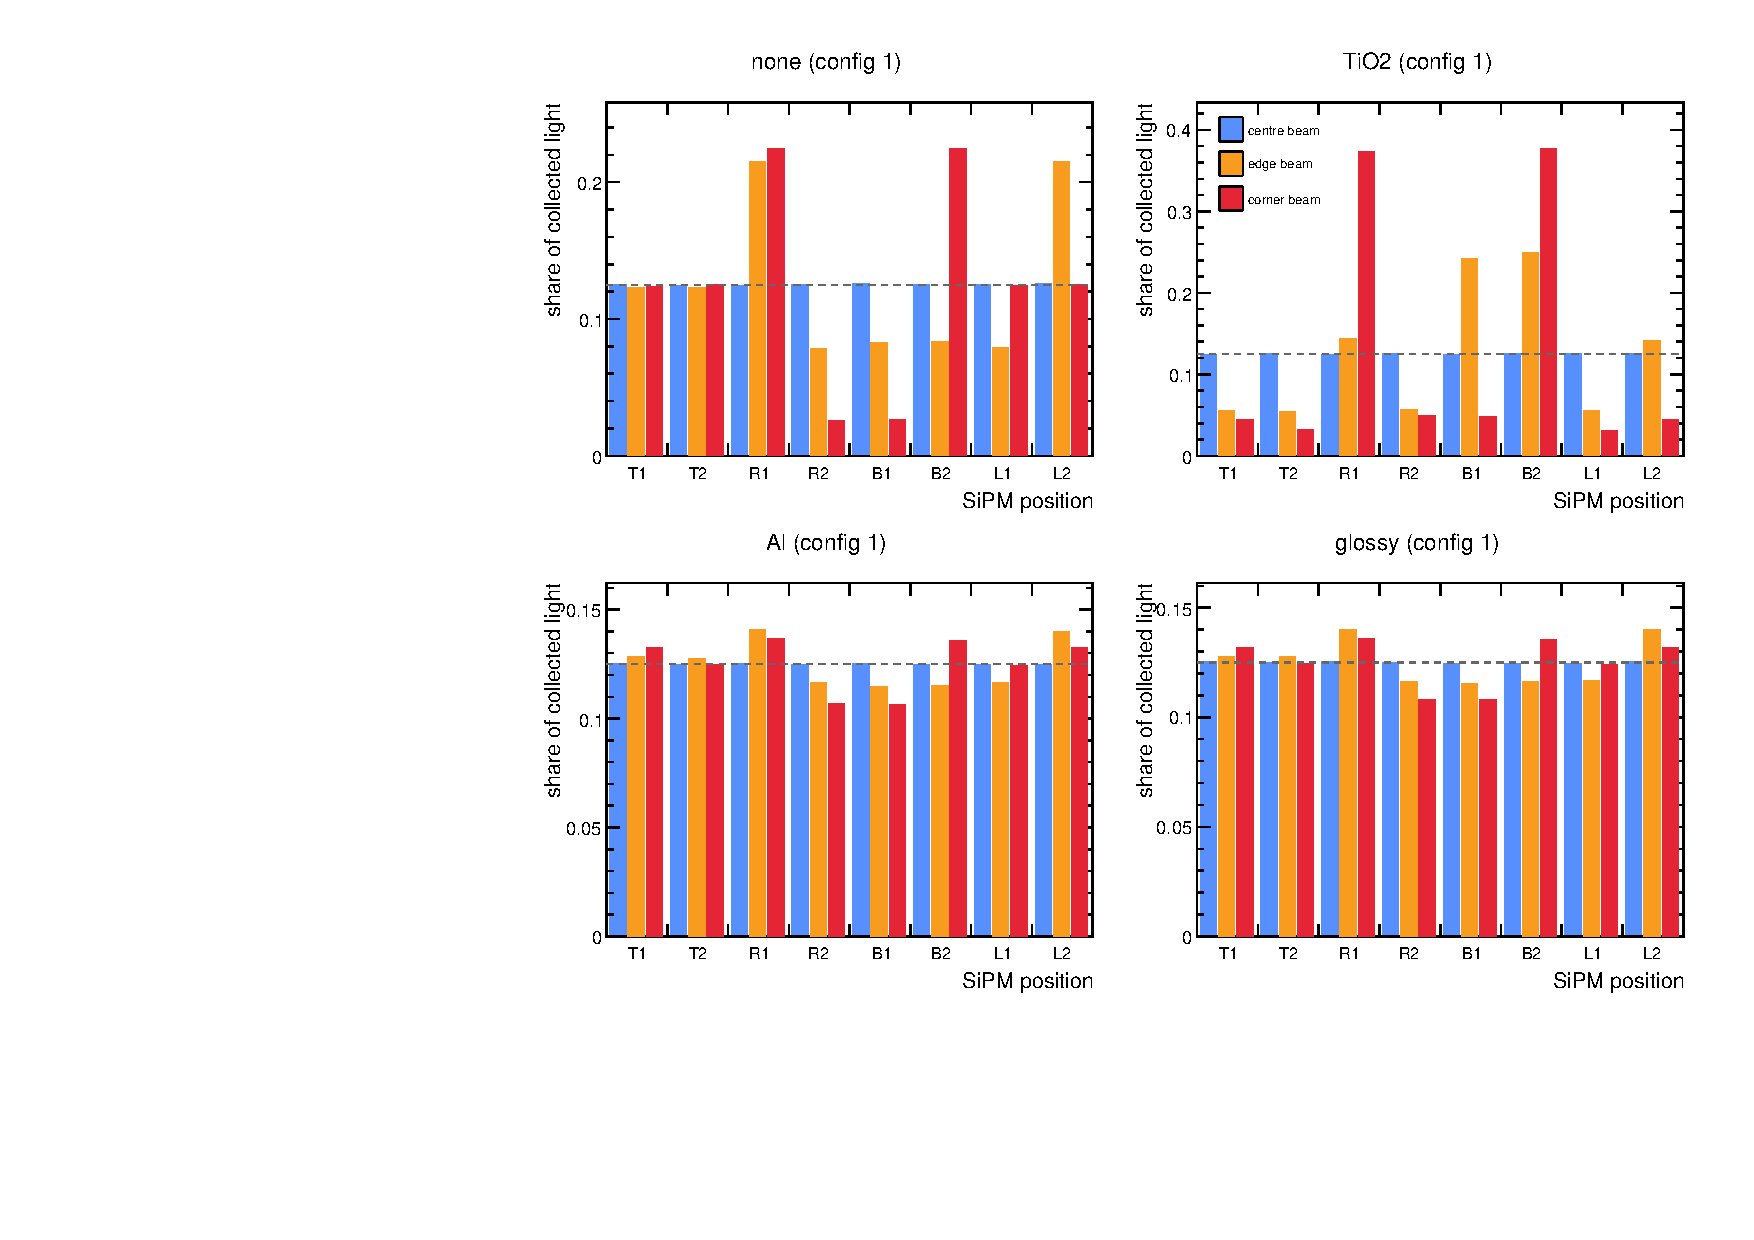
\includegraphics[width=0.7\textwidth]{fig_sipm_sharing.pdf}
\caption{Direction-resolved light sharing for Config~1, one panel per treatment.
Each group of bars is one sensor; the three colours are the irradiation
positions; the dashed line marks the uniform expectation $1/8$. For the bare
plate the light remains concentrated on the two nearest sensors, whereas the
reflective treatments distribute it almost uniformly.}
\label{fig:sharing}
\end{figure*}

\subsection{Position-resolved efficiency maps}
\label{sec:maps}

Figure~\ref{fig:grid} shows the collection efficiency as a function of the muon
entry point for Config~1, in \SI{5}{\milli\meter} cells, one panel per
treatment. Only the three irradiated patches are populated. Within a patch the
reflective treatments are nearly featureless, consistent with the uniform
integrated response found above, whereas the bare plate and, to a lesser degree,
the TiO$_2$ coating show a clear gradient across the field, brightest on the
side nearest a sensor.

\begin{figure*}[t]
\centering
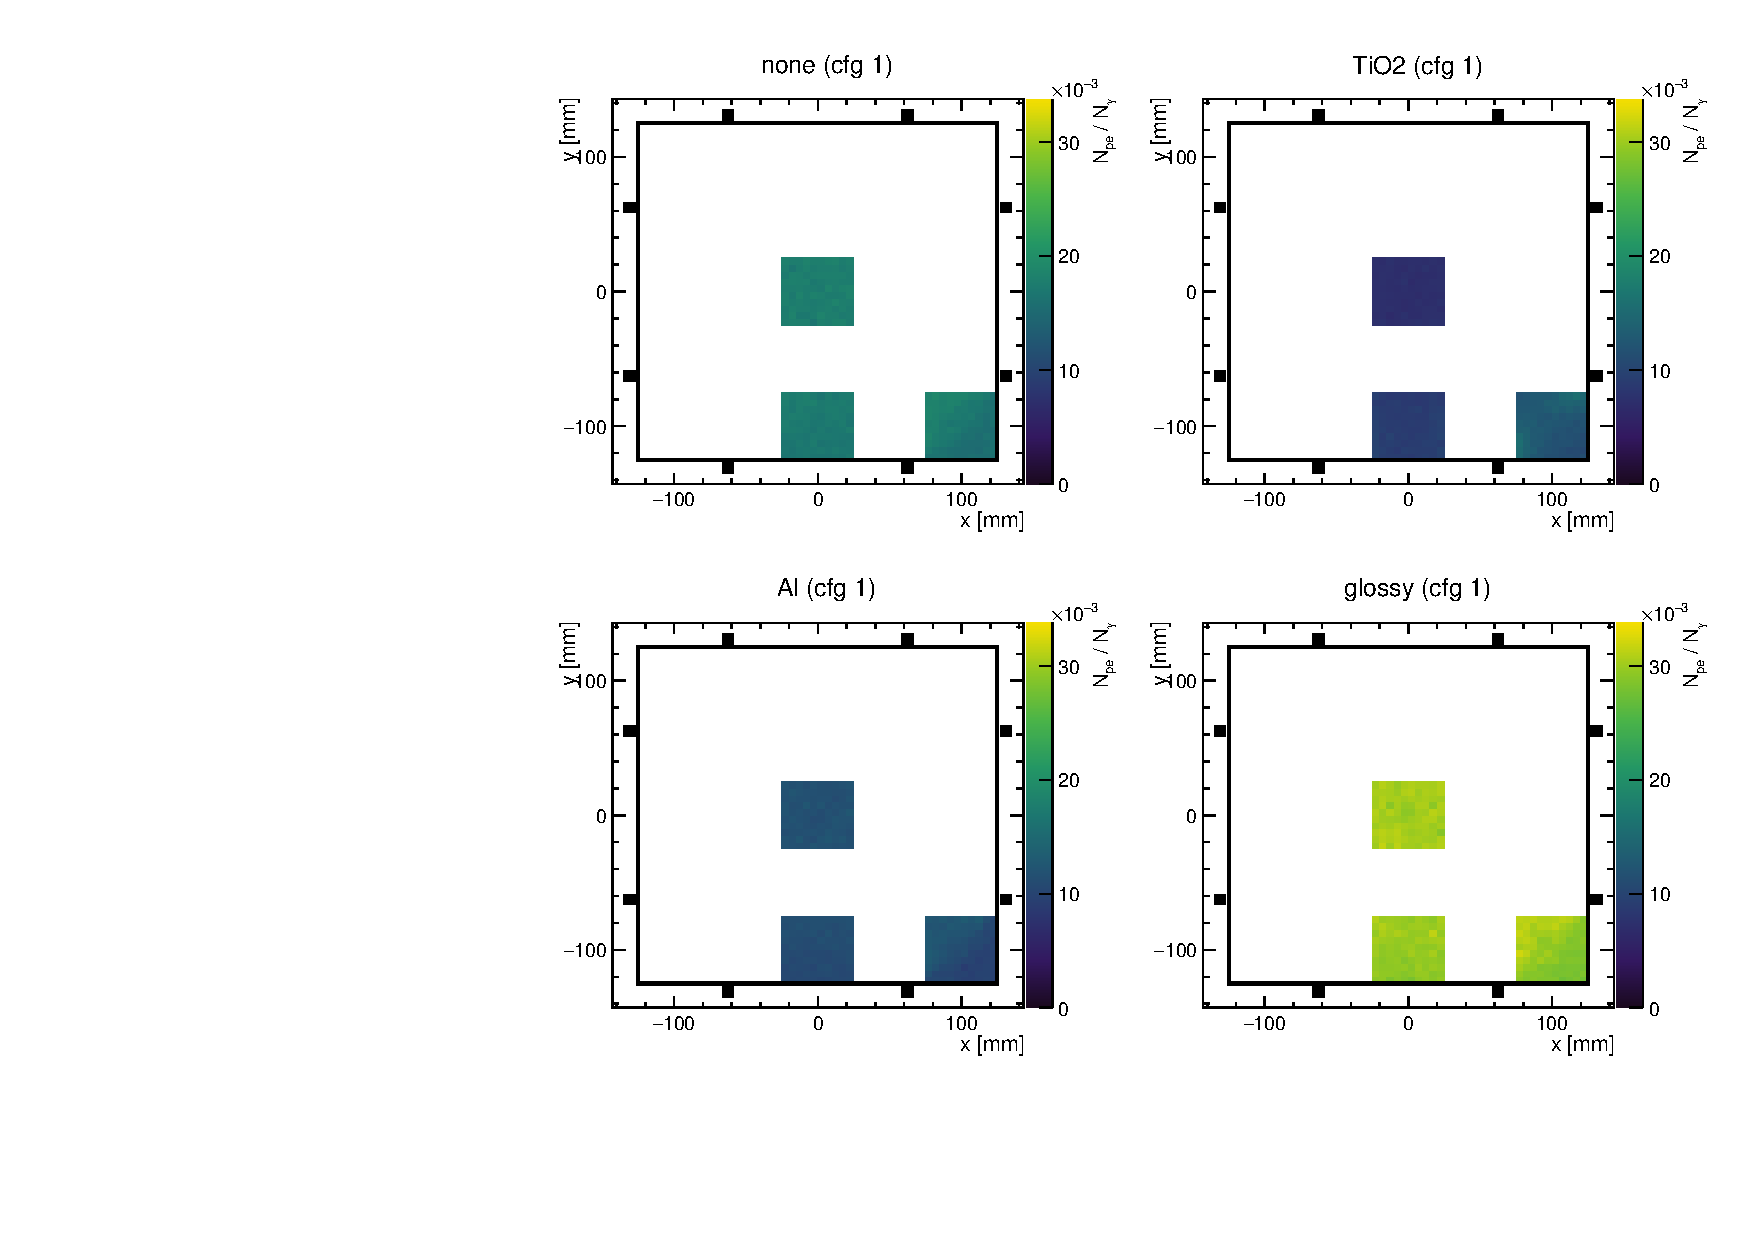
\includegraphics[width=0.7\textwidth]{efficiency_grid_cfg1_all.pdf}
\caption{Collection efficiency map for Config~1, one panel per treatment
(\SI{5}{\milli\meter} cells). Black squares mark the \sipm{} positions. The
reflective treatments are nearly uniform within each irradiated patch.}
\label{fig:grid}
\end{figure*}

\subsection{Whole-plate uniformity}
\label{sec:whole}

The three-patch scan resolves the centre, edge and corner but not the whole
plate. A second campaign irradiates the full
\SI{250}{\milli\meter}$\times$\SI{250}{\milli\meter} surface uniformly with
\num{25000} events per (layout, treatment) pair. Figure~\ref{fig:whole} shows
the resulting maps for Config~1. The bare plate exhibits a pronounced spatial
structure: the efficiency is lowest near the centre and rises towards the
instrumented edges, where photons are created close enough to a sensor-bearing
face to be detected before the frustrated-TIR loss into the black holder can
absorb them. The reflective panels reproduce the ordering of the matrix scan
with the position dependence progressively removed; for aluminium and glossy
paper the centre and the outskirts agree to better than \SI{1}{\percent}.

\begin{figure*}[t]
\centering
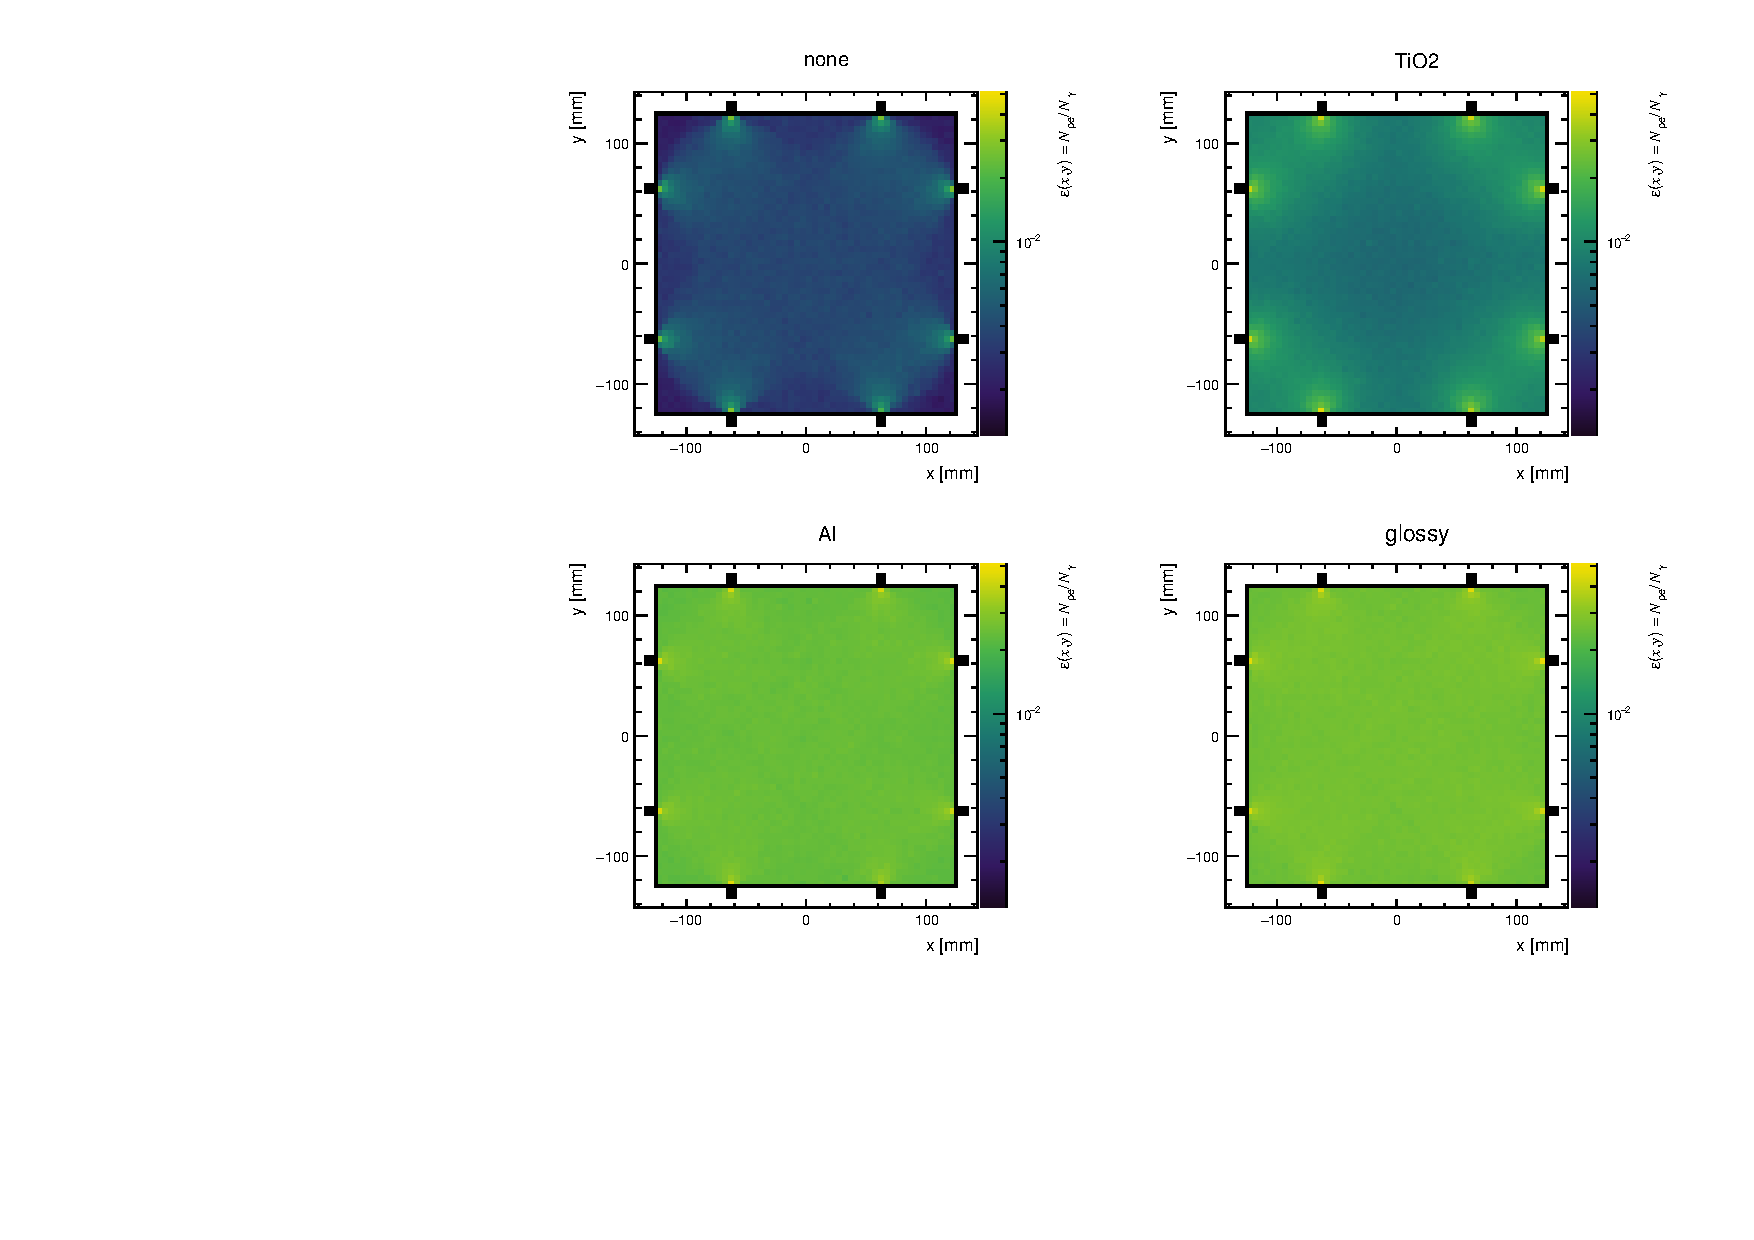
\includegraphics[width=0.7\textwidth]{whole_slab_cfg1.pdf}
\caption{Whole-plate collection-efficiency maps for Config~1 from \num{25000}
events per panel (\SI{10}{\milli\meter} cells, logarithmic colour scale). The
bare plate is dimmer at the centre and brighter towards the instrumented edges;
the reflective treatments are brighter and nearly flat.}
\label{fig:whole}
\end{figure*}

To quantify the response over the whole plate we bin the events on a
$5\times5$ grid of \SI{50}{\milli\meter} cells and form the contrast
\begin{equation}
  \kappa = \frac{\max_{\mathrm{cell}}\eps}{\min_{\mathrm{cell}}\eps},
  \label{eq:wholecontrast}
\end{equation}
so that $\kappa=1$ denotes a uniform response and $\kappa-1$ the fractional
spread over the plate. Unlike a purely radial average, this metric retains the
azimuthal information that distinguishes the single-sided layouts. The values
are listed in Table~\ref{tab:wholecontrast}. The treatments are ranked
identically and monotonically in every layout,
\begin{equation}
  \text{bare} \gg \text{TiO}_2 > \text{Al} \gtrsim \text{glossy},
  \label{eq:wholeordering}
\end{equation}
in agreement with the three-patch ordering. The whole-plate contrast is
numerically larger than the three-patch value because the full plate includes
the extreme corners that the three patches average over: $\kappa$ reaches
$15.7$ for the bare plate in Config~2 and $138$ in Config~4. The mirror-like
treatments keep $\kappa < 1.6$ in every layout. The single-sided layouts are the
discriminating case: for Config~4, whose WLS fibre runs the full length of one
edge, the near--far asymmetry across the plate is the strongest of the study,
giving the largest whole-plate contrast, whereas the four-sided layouts~(1
and~2) remain nearly uniform.

\begin{figure*}[t]
\centering
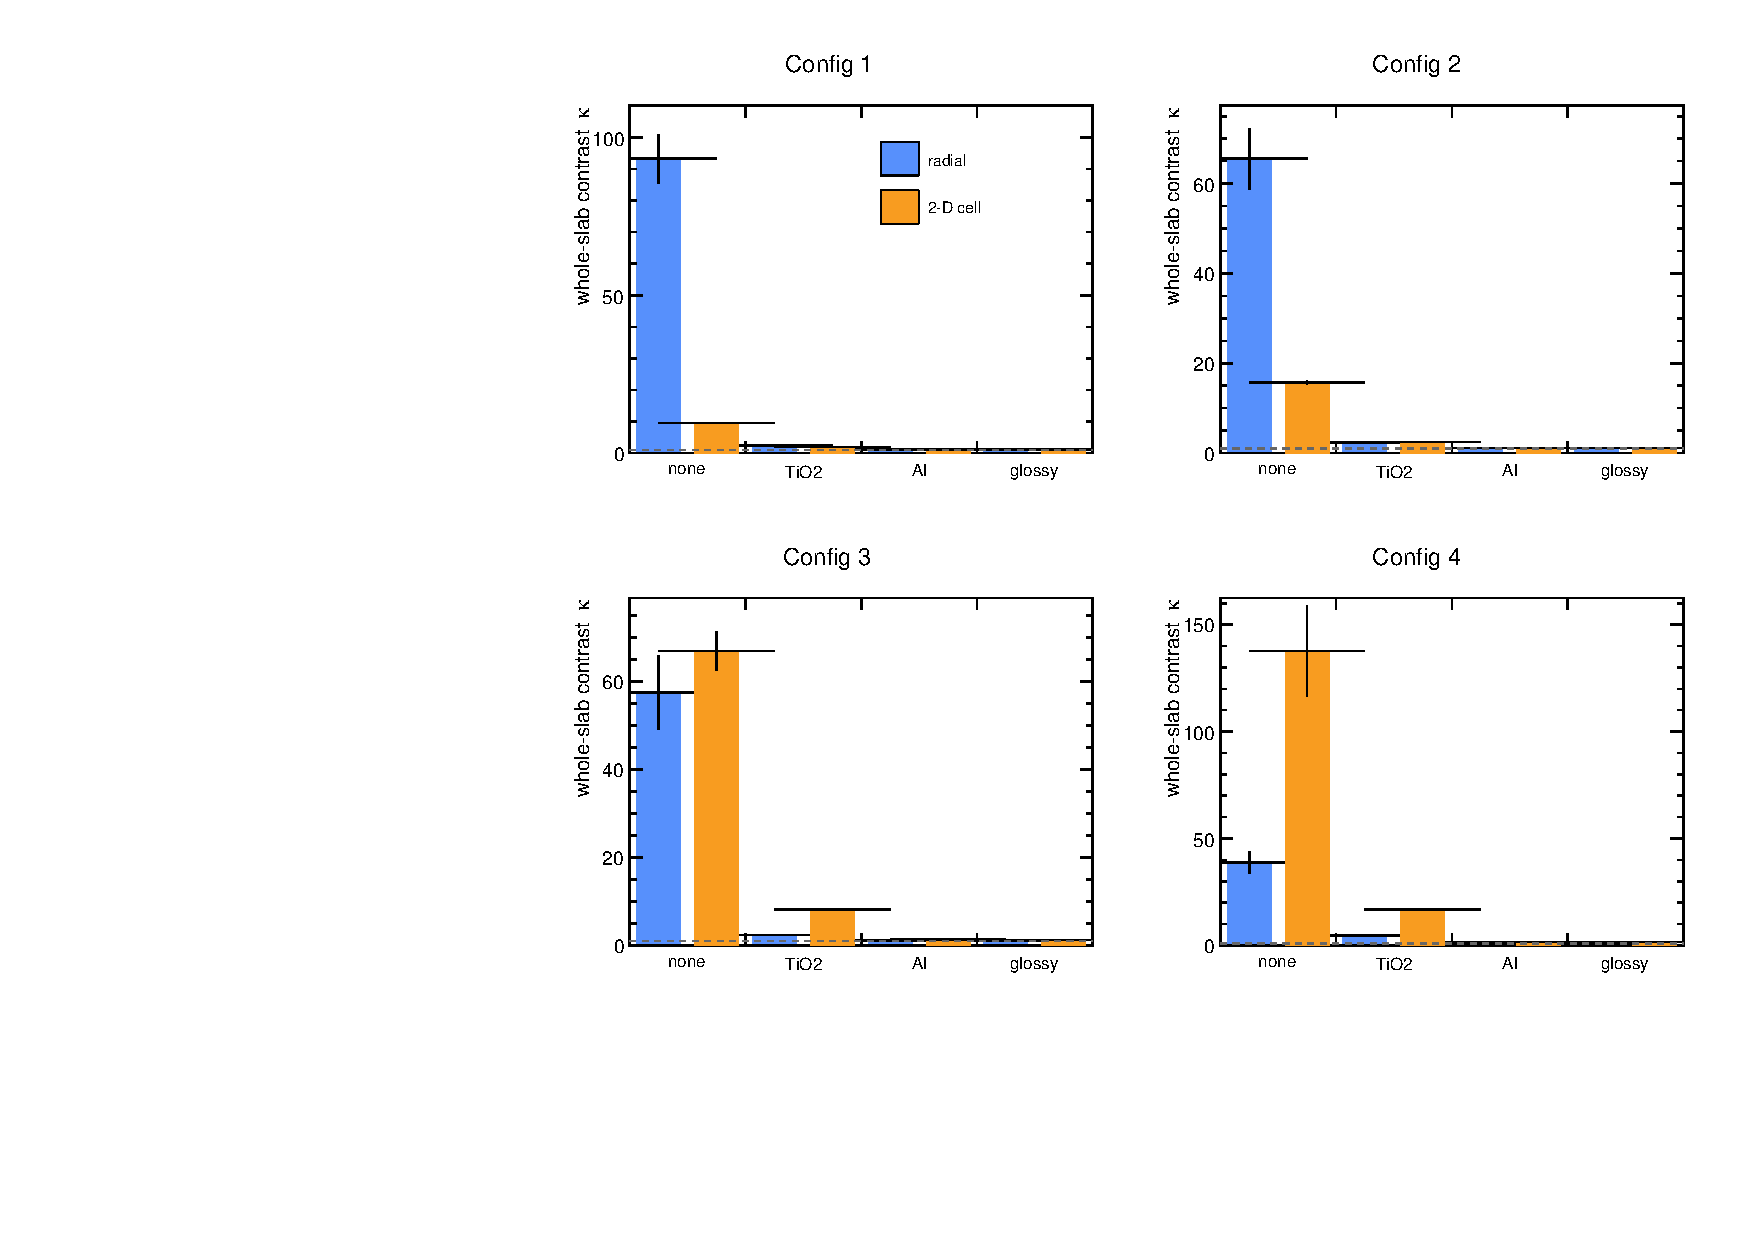
\includegraphics[width=0.6\textwidth]{fig_whole_uniformity.pdf}
\caption{Whole-plate contrast $\kappa$ (Eq.~\eqref{eq:wholecontrast}) from
\SI{50}{\milli\meter} cells, one panel per layout, four treatments per panel
(dashed line: $\kappa=1$). Both the ordering and the magnitude separate the
absorbing bare plate from the reflective treatments in every layout.}
\label{fig:wholeunif}
\end{figure*}

\begin{table}[t]
\centering
\caption{Whole-plate contrast $\kappa=\max_{\mathrm{cell}}\eps/\min_{\mathrm{cell}}\eps$
over \SI{50}{\milli\meter} cells, from \num{25000} events per
(layout, treatment) pair. A value of unity denotes a uniform response.}
\label{tab:wholecontrast}
\small
\begin{tabular}{@{}lcccc@{}}
\toprule
Treatment & Config~1 & Config~2 & Config~3 & Config~4 \\
\midrule
Bare    & 9.5 & 15.7 & 67 & 138 \\
TiO$_2$ & 1.90 & 2.47 & 8.15 & 16.9 \\
Al      & 1.08 & 1.13 & 1.29 & 1.51 \\
Glossy  & 1.06 & 1.11 & 1.24 & 1.48 \\
\bottomrule
\end{tabular}
\end{table}

% =====================================================================
\section{Discussion}
\label{sec:discussion}
% =====================================================================

\subsection{Origin of the reflector ordering}
The simulation reproduces the measured ordering
$\text{bare} \ll \text{TiO}_2 < \text{Al} \approx \text{glossy}$ and explains it
in terms of the photon-transport regime rather than in terms of a fitted
collection parameter. For the bare plate the non-instrumented faces are in
effective optical contact with a black holder whose refractive index is close to
that of the scintillator, so total internal reflection is frustrated and light
leaks into the walls; the result is the weakest response of the study and a
pronounced edge-read-out structure, in which photons created near an
instrumented face are collected before the loss to the holder can act. A
reflective treatment reverses this: photons that reach an outer face are
returned to the plate and are eventually collected, which raises the efficiency
by one to more than two orders of magnitude and, more importantly, makes the
response almost independent of the muon entry point.

The two classes of reflector differ in how they mix the light. The white paint
returns light through a purely Lambertian (diffuse) channel with no total
internal reflection, so the reflected light is randomised in direction and the
position dependence is reduced but not erased. Aluminium foil and glossy paper
are modelled as lossy specular mirrors, and a specular cavity mixes the light
far more effectively: the position contrast stays below \SI{4}{\percent} in
every layout, the whole-plate response is flat to better than \SI{1}{\percent},
and the per-sensor light sharing becomes nearly uniform. The experimental
finding that aluminium and glossy paper perform equally well, and better than
the diffuse white paint, therefore distinguishes a mirror-like treatment from a
diffusive one and is reproduced only when glossy paper is modelled as a slightly
lossier mirror rather than as a diffuser. The ordering and the homogenisation
are robust: they hold for every sensor layout, for both the three-patch and the
whole-plate campaigns, and the whole-plate contrast separates the treatments in
the same monotone order as the three-patch contrast.

\subsection{Comparison with the experimental study}
The model reproduces the qualitative features reported in Ref.~\cite{Rao2025}:
the strong suppression of the bare plate, the effective equivalence of
aluminium and glossy paper as the brightest treatments, the blue detected
spectrum near \SI{460}{\nano\meter} for direct side coupling, and the
green-shifted spectrum produced by the wavelength-shifting fibre read-out. It
also quantifies the spatial uniformity that the experiment samples only at three
positions, showing that the reflector, and not the sensor layout, governs
whether the entry point is remembered.

One quantitative comparison must be made with care. In our model the
single-\sipm{} fibre layout (Config~4) collects less light than the two-\sipm{}
direct layout (Config~3), whereas Ref.~\cite{Rao2025} reports the opposite
ordering. The two configurations are, however, not directly comparable, as
Ref.~\cite{Rao2025} itself notes: they differ in sensor count, gain and input
capacitance, and the reported Config~4 quantity is a pulse height over a
fibre-augmented effective area rather than a photoelectron count. We therefore
regard the absolute cross-configuration scale as model-dependent and do not
claim a discrepancy; the physics of the fibre read-out, namely the
wavelength-shifted and strongly position-dependent character of the collected
light, is reproduced.

\subsection{Limitations of the model}
\label{sec:limitations}
The absolute efficiencies are fixed by the assumptions of the model---the
photocathode efficiency curve, the grease coupling, and the absorbed fraction of
the tabulated reflectivities---and should not be interpreted as predictions of
absolute light yield. The robust, model-independent results are the ordering of
the treatments, the splitting into an effectively absorbing bare case and a
reflective family, and the spatial homogenisation produced by the specular
reflectors.

Two further limitations are noted. First, the diffuse white-paint configuration
shows a reversed position trend in the simulation, corner $>$ edge $>$ centre,
whereas Ref.~\cite{Rao2025} reports no such effect; since the
front-painted surface is purely Lambertian, the corner geometry can couple
diffusely scattered light into the edge sensors more efficiently, but this
prediction should be confirmed with independent simulation settings before being
interpreted physically. Second, during the production runs a rare intermittent
stall was observed in the multi-threaded optical tracking, in which a single
worker thread entered a tight loop while the others waited; the affected run was
discarded and regenerated, and all results reported here are drawn from complete
sets of files.

% =====================================================================
\section{Conclusions}
\label{sec:conclusions}
% =====================================================================

A \gfour{} optical-photon Monte Carlo model of a
\SI{250}{\milli\meter}$\times$\SI{250}{\milli\meter}$\times$\SI{10}{\milli\meter}
polished plastic scintillator read out by side-coupled \sipm{}s has been
developed and applied to a matrix of four sensor layouts and four reflector
treatments at three beam positions, together with a whole-plate scan. The model
uses the \gfour{} unified surface model, with photodetection implemented through
the wavelength-dependent photocathode efficiency at the grease--\sipm{} boundary,
and the bare plate coupled to a black holder that frustrates total internal
reflection.

The simulation reproduces the measured ordering of light collection,
$\text{bare} \ll \text{TiO}_2 < \text{Al} \approx \text{glossy}$, in every layout,
and identifies frustrated total internal reflection into the holder, rather than
the intrinsic light yield, as the cause of the weak bare response. The
specular reflectors homogenise the response far more effectively than the
diffuse paint, holding the position contrast below \SI{4}{\percent} and the
whole-plate contrast below $1.6$ while the bare plate varies by more than an
order of magnitude over the plate. The wavelength-shifting fibre read-out shifts
the mean detected wavelength from \SI{460}{\nano\meter} to \SI{485}{\nano\meter},
confirming the operation of the shifter. The validated model provides a
quantitative basis for optimising the reflector and sensor coverage of
large-area plastic-scintillator muon trigger detectors.

\section*{Declaration of competing interest}
The author declares no known competing financial interests or personal
relationships that could have appeared to influence the work reported in this
paper.

\section*{Data availability}
The simulation source code, macros and the data generated in this work are
available from the author on reasonable request.

\section*{Acknowledgements}
The author thanks the authors of Ref.~\cite{Rao2025} for the experimental study
that motivated this work. [Funding to be added.]

\bibliographystyle{elsarticle-num}
\bibliography{manuscript}

\end{document}
